\pdfoutput=1
\documentclass{article}

% =========================================================================
% NeurIPS 2026 Submission
% Workshop on Continual World Models (Idea Track: 2--4 pages)
% =========================================================================

% --- Track Configuration ---
\usepackage[preprint]{neurips_2026}


% --- Essential Packages ---
\usepackage[utf8]{inputenc}
\usepackage[T1]{fontenc}
\usepackage[colorlinks=true, linkcolor=blue, citecolor=blue, urlcolor=blue]{hyperref}
\usepackage{url}
\usepackage{booktabs}
\usepackage{amsfonts}
\usepackage{amsmath}
\usepackage{amssymb}
\usepackage{amsthm}
\usepackage{nicefrac}
\usepackage{microtype}
\usepackage{xcolor}
\usepackage{graphicx}
\usepackage{bm}
\usepackage{subcaption}

% --- TikZ Setup for Architectural Vector Schematic ---
\usepackage{tikz}
\usetikzlibrary{arrows.meta, positioning, shapes.geometric, shapes.misc, calc, fit, backgrounds}

% --- Theorem and Hypothesis Environments ---
\theoremstyle{definition}
\newtheorem{definition}{Definition}
\newtheorem{hypothesis}{Hypothesis}

% --- Spacing Adjustments for 4-Page Budget ---
\setlength{\abovedisplayskip}{3pt plus 1pt minus 1pt}
\setlength{\belowdisplayskip}{3pt plus 1pt minus 1pt}
\setlength{\abovedisplayshortskip}{1pt plus 1pt minus 1pt}
\setlength{\belowdisplayshortskip}{1pt plus 1pt minus 1pt}
\setlength{\textfloatsep}{5pt plus 1pt minus 1pt}
\setlength{\floatsep}{5pt plus 1pt minus 1pt}
\setlength{\intextsep}{5pt plus 1pt minus 1pt}

% --- Title ---
\title{Toward Continually Growing World Models:\\An OaK-Inspired Architecture for Learned Abstraction and Planning}

% --- Author Block ---
\author{%
  An Xu\thanks{Idea Track paper submitted to the NeurIPS 2026 Workshop on Continual World Models.} \\
  Technical University of Munich \\
  Harbin, China \\
  \texttt{AnX.RTL2324@tum-asia.edu.sg} \\
}

\begin{document}

\maketitle

% =========================================================================
% Abstract
% =========================================================================
\begin{abstract}
Learned world models increasingly empower autonomous agents to predict transitions, imagine rollouts, and plan behaviors in complex environments. However, conventional continual world modeling paradigms predominantly formulate lifelong adaptation along a single parametric axis: updating neural network weights ($\theta_t \to \theta_{t+1}$) over a static, fixed-dimensional latent substrate and a fixed single-step temporal granularity. When deployed in non-stationary or open-ended environments, this parameter-only adaptation is vulnerable to loss of plasticity, capacity saturation, and compounding rollout errors over extended horizons. In this position paper, we argue that genuine continual world modeling requires introducing a second, structural adaptation axis ($\mathcal{K}_t \to \mathcal{K}_{t+1}$), wherein the model's predictive state abstractions, temporal abstractions, and option models continually grow, evaluate, and reorganize over time. Grounding this dual-axis formulation in Richard Sutton's OaK architecture and its \mbox{FC-STOMP} lifecycle (Feature Construction $\rightarrow$ SubTask $\rightarrow$ Option $\rightarrow$ Model $\rightarrow$ Planning), we formulate \emph{Structural Continual World Modeling} (SCWM). Under SCWM, discovered state features dynamically expand the world model's predictive state representation, inducing reward-respecting subtasks, closed-loop options, and predictive option models, with retention and pruning governed by downstream planning utility. We formulate five falsifiable research hypotheses and an experimental agenda to guide the development of continually growing world models.
\end{abstract}



% =========================================================================
% Section 1: Introduction
% =========================================================================
\section{Introduction}
\label{sec:introduction}

Model-based reinforcement learning (MBRL) with learned latent world models has demonstrated notable success across visual continuous control and robotics~\citep{ha2018world, hafner2019learning, hafner2020dream, hafner2023mastering, hansen2024tdmpc2, richens2025general}, synthesizing imagined trajectories in latent space for sample-efficient policy optimization and model predictive control (MPC).

Despite their predictive power, many modern world models retain a fixed representational topology and temporal formulation after model design/training. Practitioners fix a latent dimensionality $z_t \in \mathcal{Z} = \mathbb{R}^{d_z}$ and train single-step forward dynamics $p_\theta(z_{t+1}, r_{t+1} \mid z_t, a_t)$ over primitive actions $a_t \in \mathcal{A}$. A dominant formulation in continual world modeling focuses on parameter adaptation within a fixed predictive architecture: $\theta_{t+1} = \operatorname{Opt}(\theta_t, \mathcal{D}_{\text{new}})$~\citep{kessler2023effectiveness, yang2024augmenting, liu2025continual}.

However, this parameter-only view fails under qualitative distribution shifts. Under the \emph{Big World Hypothesis}~\citep{javed2024bigworld, lewandowski2025world, elelimy2025rethinking}, the physical world is vastly larger than any bounded agent; no pre-allocated latent representation or single temporal scale can encapsulate all future interactions. Forcing continual adaptation solely through gradient weight adjustments in a static network precipitates \emph{loss of plasticity}~\citep{dohare2024loss} and catastrophic forgetting~\citep{fu2025knowledge}. Furthermore, single-step rollouts ($z_t \to \dots \to z_{t+H}$) suffer from compounding errors and exponential search complexity over long horizons~\citep{freed2023learning, jiralerspong2023forecaster}.

We advocate that continual world modeling requires expanding beyond the parameter adaptation axis ($\theta_t \to \theta_{t+1}$) to encompass a \textbf{structural adaptation axis} ($\mathcal{K}_t \to \mathcal{K}_{t+1}$). Rather than merely re-tuning weights, the world model must continually discover, evaluate, and prune predictive abstractions across state and time. Grounding this dual-axis vision in Sutton's \textbf{OaK architecture}~\citep{sutton2025oak}---which synthesizes the Alberta Plan~\citep{sutton2022alberta}, reward-respecting subtasks~\citep{sutton2023subtasks}, constructive representations~\citep{javed2023constructive, javed2019meta}, and options~\citep{sutton1999between, sutton1998intra} into the \textbf{FC-STOMP} progression---we formulate \textbf{Structural Continual World Modeling} (SCWM).

\paragraph{Key Contributions.}
\textbf{(1) Dual-Axis Framework:} We formalize SCWM, augmenting parameter-level adaptation ($\theta_t \to \theta_{t+1}$) with an explicit structural adaptation axis $(\theta_t, \mathcal{K}_t) \to (\theta_{t+1}, \mathcal{K}_{t+1})$.
\textbf{(2) Constructive Dynamics:} We formalize how discovered features $\mathcal{F}_t$ directly expand the world model's predictive state representation ($\tilde{z}_t = \Phi_t(z_t)$), inducing reward-respecting subtasks with terminal stopping bonuses, predictive option models, and multi-scale planning.
\textbf{(3) Actionable Agenda:} We formulate five falsifiable hypotheses (H1--H5) and experimental protocols evaluating planning depth, plasticity retention, and Pareto-optimal utility pruning.

% =========================================================================
% Section 2: Beyond Parameter-Level Continual World Modeling
% =========================================================================
\section{Beyond Parameter-Level Continual World Modeling}
\label{sec:gap}
\enlargethispage{1.5\baselineskip}

Standard continual world modeling formalizes adaptation as parameter trajectory estimation under a stationary architecture:
\begin{equation}
\label{eq:param_update}
\theta_{t+1} = \arg\min_\theta \mathbb{E}_{(o, a, o') \sim \mathcal{D}_{\text{new}}} \left[ \mathcal{L}_{\text{WM}}(M_\theta(E_\phi(o), a), o') \right] + \Omega(\theta, \theta_t),
\end{equation}
where $\Omega$ regularizes weight drift or penalizes rehearsal divergence~\citep{kessler2023effectiveness, yang2024augmenting}. We identify three fundamental structural bottlenecks:
\textbf{1. Fixed Representational Topology:} The encoder $E_\phi: \Omega \to \mathcal{Z}$ enforces a fixed coordinate dimensionality $\mathcal{Z} \subset \mathbb{R}^{d_z}$, unable to dynamically allocate additional predictive dimensions for novel interaction affordances.
\textbf{2. Fixed Temporal Granularity:} Single-step dynamics $(z_t, a_t) \mapsto z_{t+1}$ require autoregressive rollouts $\hat{z}_{t+H} \sim \prod_{k=0}^{H-1} p_\theta(z_{t+k+1} \mid z_{t+k}, a_{t+k})$, compounding approximation errors and exploding search over $\mathcal{A}^H$~\citep{freed2023learning, jiralerspong2023forecaster}.
\textbf{3. Capacity Saturation:} Sustained non-stationary gradient updates cause unit saturation, gradient rank collapse, and plasticity decay~\citep{dohare2024loss}.

\begin{definition}[\textbf{Structural Continual World Modeling}]
\label{def:scwm}
A \emph{Structural Continual World Model} is defined by $\mathcal{W}_t = (\theta_t, \mathcal{K}_t)$, where $\theta_t$ denotes continuous parameters and $\mathcal{K}_t = (\mathcal{F}_t, \mathcal{G}_t, \mathcal{O}_t, \mathcal{M}_t)$ is a knowledge structure comprising:
constructed features $\mathcal{F}_t = \{f_i: \mathcal{Z} \to \mathbb{R}\}$, subtasks $\mathcal{G}_t$, closed-loop options $\mathcal{O}_t = \{o_i = (\mathcal{I}_i, \pi_i, \beta_i)\}$, and predictive option models $\mathcal{M}_t = \{\mathcal{M}_{o_i}\}$.
The predictive state representation $\tilde{z}_t \in \tilde{\mathcal{Z}}_t$ dynamically expands with $\mathcal{F}_t$:
\begin{equation}
\label{eq:expanded_state}
\tilde{z}_t = \Phi_t(z_t) \triangleq \left[ z_t^\top, \; f_1(z_t), \; \dots, \; f_{|\mathcal{F}_t|}(z_t) \right]^\top \in \mathbb{R}^{d_z + |\mathcal{F}_t|}.
\end{equation}
Lifelong learning is governed by joint parameter adaptation and structural knowledge evolution:
\begin{equation}
\label{eq:structural_transition}
(\theta_t, \mathcal{K}_t) \xrightarrow{\text{Experience } e_{t:t+\Delta}} (\theta_{t+1}, \mathcal{K}_{t+1}), \quad \text{where } \mathcal{K}_{t+1} \neq \mathcal{K}_t \text{ in general}.
\end{equation}
\end{definition}

% =========================================================================
% Section 3: An OaK-Inspired Continually Growing World Model
% =========================================================================
\section{An OaK-Inspired Continually Growing World Model}
\label{sec:architecture}

\begin{figure*}[t]
\centering
\vspace{-0.15cm}
\resizebox{\textwidth}{!}{%
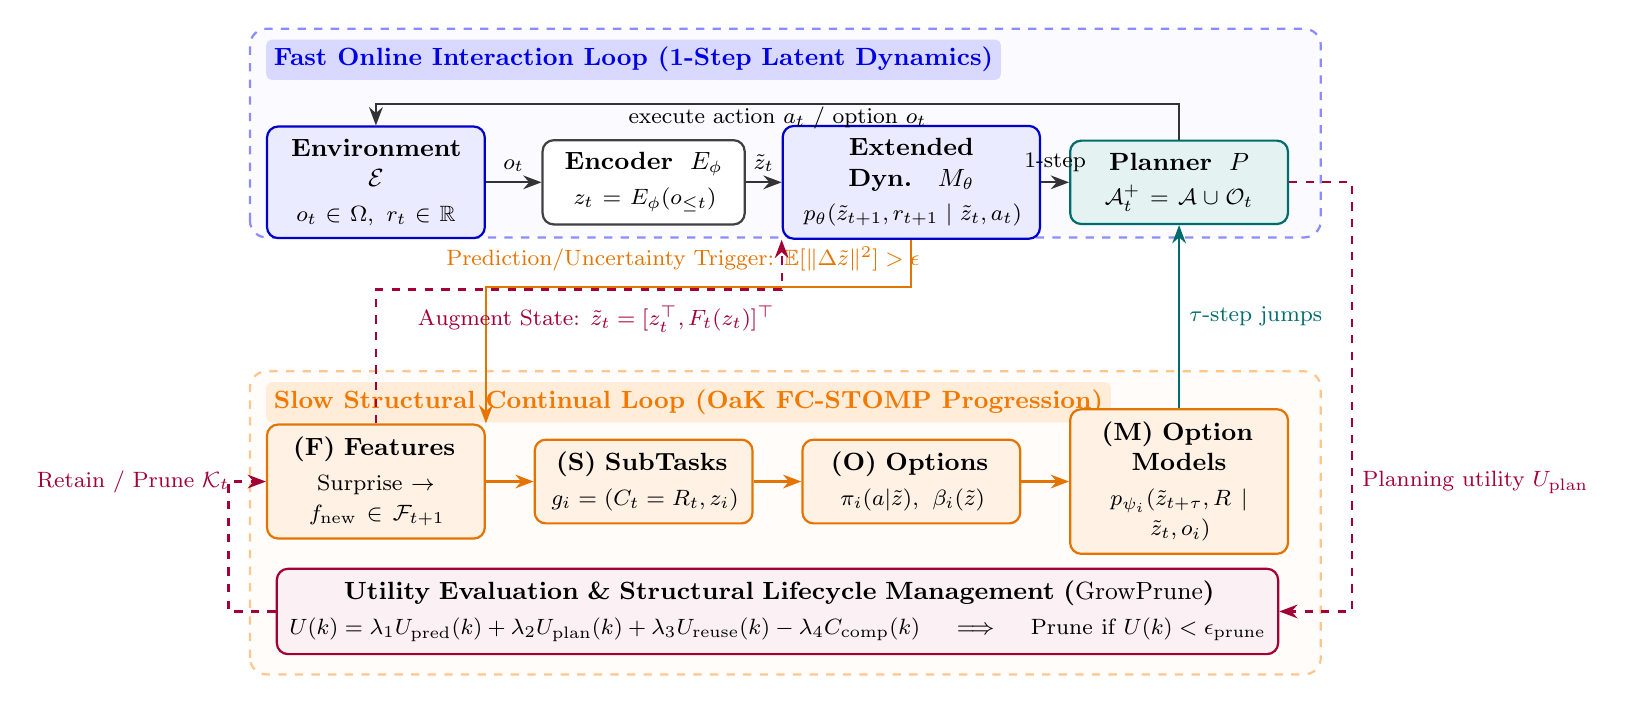
\begin{tikzpicture}[
    >=Stealth,
    box/.style={rectangle, draw=black!75, thick, rounded corners=4pt, align=center, fill=white, inner sep=4.5pt, font=\small},
    databox/.style={rectangle, draw=blue!80!black, thick, rounded corners=4pt, align=center, fill=blue!8, inner sep=4.5pt, font=\small},
    oakbox/.style={rectangle, draw=orange!90!black, thick, rounded corners=4pt, align=center, fill=orange!10, inner sep=4.5pt, font=\small},
    planbox/.style={rectangle, draw=teal!85!black, thick, rounded corners=4pt, align=center, fill=teal!10, inner sep=4.5pt, font=\small},
    arrow/.style={->, thick, draw=black!80},
    oakarrow/.style={->, thick, draw=orange!90!black},
    looparrow/.style={->, thick, dashed, draw=purple!85!black}
]

% =============================================================
% Background Framing Panels & Titles (Anchored to top-left)
% =============================================================
% Top Panel: Fast Base Dynamics Loop
\draw[draw=blue!45, fill=blue!2, dashed, thick, rounded corners=6pt] (-0.3, 5.2) rectangle (13.3, 7.85);
\node[anchor=north west, fill=blue!15, text=blue!90!black, font=\small\bfseries, rounded corners=2pt, inner sep=2.8pt] at (-0.1, 7.72) {Fast Online Interaction Loop (1-Step Latent Dynamics)};

% Bottom Panel: Slow Structural Adaptation Loop
\draw[draw=orange!45, fill=orange!2, dashed, thick, rounded corners=6pt] (-0.3, -0.35) rectangle (13.3, 3.5);
\node[anchor=north west, fill=orange!15, text=orange!95!black, font=\small\bfseries, rounded corners=2pt, inner sep=2.8pt] at (-0.1, 3.37) {Slow Structural Continual Loop (OaK FC-STOMP Progression)};

% =============================================================
% Row 1: Fast Base Dynamics (y = 5.9)
% =============================================================
\node[databox, text width=2.45cm] (env) at (1.3, 5.9) {\textbf{Environment } $\mathcal{E}$\\\vspace{1.5pt}{\footnotesize $o_t \in \Omega,\; r_t \in \mathbb{R}$}};
\node[box, text width=2.25cm] (enc) at (4.7, 5.9) {\textbf{Encoder } $E_\phi$\\\vspace{1.5pt}{\footnotesize $z_t = E_\phi(o_{\le t})$}};
\node[databox, text width=2.95cm] (wm) at (8.1, 5.9) {\textbf{Extended Dyn. } $M_\theta$\\\vspace{1.5pt}{\footnotesize $p_\theta(\tilde{z}_{t+1}, r_{t+1} \mid \tilde{z}_t, a_t)$}};
\node[planbox, text width=2.45cm] (plan) at (11.5, 5.9) {\textbf{Planner } $P$\\\vspace{1.5pt}{\footnotesize $\mathcal{A}^+_t = \mathcal{A} \cup \mathcal{O}_t$}};

% Horizontal Fast Loop Connections
\draw[arrow] (env) -- node[above, font=\footnotesize] {$o_t$} (enc);
\draw[arrow] (enc) -- node[above, font=\footnotesize] {$\tilde{z}_t$} (wm);
\draw[arrow] (wm) -- node[above, font=\footnotesize] {$1$-step} (plan);
\draw[arrow] (plan.north) -- ++(0, 0.45) -| (env.north);
\node[font=\footnotesize, anchor=south] at (6.4, 6.45) {execute action $a_t$ / option $o_t$};

% =============================================================
% Row 2: Slow Structural OaK Progression (y = 2.1)
% =============================================================
\node[oakbox, text width=2.45cm] (fc) at (1.3, 2.1) {\textbf{(F) Features}\\\vspace{1.5pt}{\footnotesize Surprise $\to f_{\text{new}} \in \mathcal{F}_{t+1}$}};
\node[oakbox, text width=2.45cm] (subtask) at (4.7, 2.1) {\textbf{(S) SubTasks}\\\vspace{1.5pt}{\footnotesize $g_i = (C_t=R_t, z_i)$}};
\node[oakbox, text width=2.45cm] (option) at (8.1, 2.1) {\textbf{(O) Options}\\\vspace{1.5pt}{\footnotesize $\pi_i(a|\tilde{z}),\; \beta_i(\tilde{z})$}};
\node[oakbox, text width=2.45cm] (optmodel) at (11.5, 2.1) {\textbf{(M) Option Models}\\\vspace{1.5pt}{\footnotesize $p_{\psi_i}(\tilde{z}_{t+\tau}, R \mid \tilde{z}_t, o_i)$}};

% Horizontal OaK Pipeline
\draw[oakarrow] (fc) -- (subtask);
\draw[oakarrow] (subtask) -- (option);
\draw[oakarrow] (option) -- (optmodel);

% Cross-Loop Structural Channels (Centered, zero collision)
% =============================================================
% Surprise Trigger (Drop from wm to fc)
\draw[oakarrow] (wm.south) -- ++(0, -0.6) -| (fc.north east);
\node[font=\footnotesize, color=orange!90!black, anchor=south] at (5.2, 4.65) {Prediction/Uncertainty Trigger: $\mathbb{E}[\|\Delta \tilde{z}\|^2] > \epsilon$};

% State Augmentation (Rise from fc to wm)
\draw[looparrow] (fc.north) -- ++(0, 1.7) -| (wm.south west);
\node[font=\footnotesize, color=purple!85!black, anchor=north] at (4.1, 4.45) {Augment State: $\tilde{z}_t = [z_t^\top, F_t(z_t)]^\top$};

% Option Model Supply to Planner (Far right)
\draw[->, thick, draw=teal!85!black] (optmodel.north) -- node[right, font=\footnotesize, color=teal!85!black] {$\tau$-step jumps} (plan.south);

% =============================================================
% Row 3: Utility Evaluation & Structural Pruning (y = 0.45)
% =============================================================
\node[box, draw=purple!85!black, fill=purple!6, text width=12.4cm] (utility) at (6.4, 0.45) {\textbf{Utility Evaluation \& Structural Lifecycle Management ($\operatorname{GrowPrune}$)}\\\vspace{1.5pt}{\footnotesize $U(k) = \lambda_1 U_{\text{pred}}(k) + \lambda_2 U_{\text{plan}}(k) + \lambda_3 U_{\text{reuse}}(k) - \lambda_4 C_{\text{comp}}(k) \quad \implies \quad \text{Prune if } U(k) < \epsilon_{\text{prune}}$}};

% Utility Feedback Channels
\draw[looparrow] (plan.east) -- ++(0.8, 0) |- node[right, pos=0.35, font=\footnotesize, color=purple!85!black] {Planning utility $U_{\text{plan}}$} (utility.east);
\draw[looparrow] (utility.west) -- ++(-0.6, 0) |- node[left, pos=0.65, font=\footnotesize, color=purple!85!black] {Retain / Prune $\mathcal{K}_t$} (fc.west);

\end{tikzpicture}%
}
\vspace{-0.25cm}
\caption{\textbf{Architectural overview of the OaK-inspired Continually Growing World Model.} A \emph{Fast Base Dynamics Loop} handles 1-step primitive predictions over the extended state $\tilde{z}_t$, coupled with a \emph{Slow Structural Adaptation Loop} executing the OaK FC-STOMP cycle. Systematic prediction surprises trigger feature construction ($F$), expanding $\tilde{z}_t$ and inducing subtasks ($S$), options ($O$), and predictive option models ($M$). Multi-scale planning ($P$) leverages both primitive and abstract transitions, returning empirical planning utility to retain or prune components.}
\label{fig:oak_wm_arch}
\vspace{-0.25cm}
\end{figure*}

We instantiate Definition~\ref{def:scwm} by systematically operationalizing Sutton's FC-STOMP lifecycle~\citep{sutton2025oak} into latent world models (Figure~\ref{fig:oak_wm_arch}, Table~\ref{tab:oak_mapping}).

\subsection{Base Latent Dynamics Foundation}
{\setlength{\abovedisplayskip}{3pt}\setlength{\belowdisplayskip}{3pt}
Given observation stream $o_{\le t}$, base encoder $E_\phi$ extracts belief embedding $z_t = E_\phi(o_{\le t})$. Incorporating discovered features $\mathcal{F}_t$, the world model operates over the extended predictive state $\tilde{z}_t = \Phi_t(z_t) \in \mathbb{R}^{d_z + |\mathcal{F}_t|}$ (Eq.~\ref{eq:expanded_state}), predicting 1-step transitions and rewards: $\hat{\tilde{z}}_{t+1}, \hat{r}_{t+1} \sim p_{\theta, t}(\tilde{z}_{t+1}, r_{t+1} \mid \tilde{z}_t, a_t)$ for $a_t \in \mathcal{A}$.

\subsection{Continual Feature Construction \texorpdfstring{($F$)}{(F)}}
\enlargethispage{1.8\baselineskip}
When systematic prediction surprises or epistemic uncertainties exceed a cognitive threshold ($\mathbb{E}[\|\tilde{z}_{t+1} - \hat{\tilde{z}}_{t+1}\|^2] > \epsilon_{\text{trigger}}$), candidate feature functions $f_{\text{new}}: \mathcal{Z} \to \mathbb{R}$ are generated:
\begin{equation}
\label{eq:feature_generation}
f_i(z_t) = \sigma\left(\bm{w}_i^\top \psi(z_t) + b_i\right), \quad \mathcal{F}_{t+1} = \mathcal{F}_t \cup \{f_{\text{new}}\},
\end{equation}
where $\psi(z_t)$ represents constructive hidden units~\citep{javed2023constructive, kearney2019learning}. Adding $f_{\text{new}}$ expands $\tilde{z}_t \to \tilde{z}_t^{(t+1)}$, structurally expanding the computational basis of the predictive state representation. Extending structural construction to recover predictive information omitted by the base encoder remains an important open problem.

\subsection{Reward-Respecting Subtasks \texorpdfstring{($S$)}{(S)} and Options \texorpdfstring{($O$)}{(O)}}
Following Sutton et al.~\citep{sutton2023subtasks}, each constructed feature $f_i \in \mathcal{F}_t$ induces a \emph{reward-respecting subtask} $g_i = (C_t = R_t, z_i) \in \mathcal{G}_t$. The subtask preserves environmental reward $C_t = R_t$ as its ongoing cumulant, combined with a terminal stopping bonus upon option termination:
\begin{equation}
\label{eq:reward_respecting_subtask}
z_i(\tilde{z}_{\text{term}}) = \hat{v}(\tilde{z}_{\text{term}}) + (\bar{w}_i - w_i) f_i(z_{\text{term}}),
\end{equation}
where $\hat{v}(\tilde{z})$ is the baseline value estimate and $(\bar{w}_i - w_i)$ modulates feature attainment. Solving subtask $g_i$ yields an option $o_i = (\mathcal{I}_i, \pi_i, \beta_i) \in \mathcal{O}_t$~\citep{sutton1999between}, where $\pi_i(a \mid \tilde{z})$ is the policy, $\beta_i(\tilde{z}) \in [0, 1]$ is the termination condition, and one natural choice for initiation set is $\mathcal{I}_i = \{\tilde{z} \mid f_i(z) \ge \delta_{\text{init}}\}$.

\subsection{Predictive Option Models \texorpdfstring{($M$)}{(M)}}
For each option $o_i \in \mathcal{O}_t$, the agent fits a multi-step jump-ahead transition and cumulative return model $\mathcal{M}_{o_i} \in \mathcal{M}_t$ over extended states~\citep{sutton1998intra, freed2023learning, rodriguez2024learning}:
\begin{equation}
\label{eq:option_model}
\mathcal{M}_{o_i}: (\tilde{z}_t, o_i) \mapsto (\hat{\tilde{z}}_{t+\tau}, \hat{R}_{t:t+\tau}, \hat{\tau}) \sim p_{\psi_i}(\tilde{z}_{t+\tau}, R_{t:t+\tau}, \tau \mid \tilde{z}_t, o_i),
\end{equation}
where $\tau \in \mathbb{N}_{\ge 1}$ is duration and $R_{t:t+\tau} = \sum_{k=0}^{\tau-1} \gamma^k r_{t+k+1}$ is cumulative return, trained off-policy via intra-option model learning~\citep{sutton1998intra}.

\subsection{Planning Across Temporal Scales \texorpdfstring{($P$)}{(P)}}
The planner searches over hybrid action space $\mathcal{A}^+_t = \mathcal{A} \cup \mathcal{O}_t$, traversing primitive steps and multi-step jumps ($\tilde{z}_0 \xrightarrow{a_0} \dots \xrightarrow{o_k} \tilde{z}_{t+H}$), contracting graph diameter for deep horizon search~\citep{jiralerspong2023forecaster, precup1997planning}.
}

\begin{table*}[t]
\centering
\vspace{-0.25cm}
\caption{\textbf{Mapping Sutton's OaK FC-STOMP Lifecycle to Structural Continual World Models.}}
\label{tab:oak_mapping}
\footnotesize
\renewcommand{\arraystretch}{0.82}
\resizebox{0.86\textwidth}{!}{%
\begin{tabular}{lll}
\toprule
\textbf{OaK Component} & \textbf{World-Model Interpretation} & \textbf{Formal Representation / Mechanism} \\
\midrule
\textbf{Base Substrate} & Parametric latent dynamics baseline & $z_t = E_\phi(o_{\le t}), \;\; p_\theta(\tilde{z}_{t+1}, r_{t+1} \mid \tilde{z}_t, a_t)$ \\
\textbf{Feature Construction ($F$)} & Predictive state representation expansion & $\mathcal{F}_{t+1} = \mathcal{F}_t \cup \{f_{\text{new}}\}, \;\; \tilde{z}_t = [z_t^\top, f_1(z_t), \dots]^\top$ \\
\textbf{SubTask ($S$)} & Reward-respecting local control objective & $\mathcal{G}_{t+1} = \mathcal{G}_t \cup \{g_i\}, \;\; g_i = (C_t = R_t, z_i)$ \\
\textbf{Option ($O$)} & Closed-loop temporally extended behavior & $\mathcal{O}_{t+1} = \mathcal{O}_t \cup \{o_i\}, \;\; o_i = (\mathcal{I}_i, \pi_i, \beta_i)$ \\
\textbf{Option Model ($M$)} & Temporal jump-ahead predictive dynamics & $\mathcal{M}_{o_i}: (\tilde{z}_t, o_i) \mapsto (\hat{\tilde{z}}_{t+\tau}, \hat{R}_{t:t+\tau}, \hat{\tau}) \sim p_{\psi_i}$ \\
\textbf{Planning ($P$)} & Multi-scale forward tree/trajectory search & $\mathcal{A}^+_t = \mathcal{A} \cup \mathcal{O}_t, \;\; \text{Search over hybrid rollouts}$ \\
\textbf{Utility Feedback} & Knowledge retention, revision, and pruning & $U(k) = \lambda_1 U_{\text{pred}} + \lambda_2 U_{\text{plan}} + \lambda_3 U_{\text{reuse}} - \lambda_4 C_{\text{comp}}$ \\
\bottomrule
\end{tabular}%
}
\vspace{-0.15cm}
\end{table*}

\subsection{Utility-Driven Growth and Pruning: Managing Complexity}
\enlargethispage{1.8\baselineskip}
To balance capacity and avoid search explosion in $\mathcal{A}^+_t$, abstraction utility $U(k)$ (Table~\ref{tab:oak_mapping}) is audited across accuracy, planning utility, and reuse. Low-utility elements ($U(k) < \epsilon_{\text{prune}}$) are pruned: $\mathcal{K}_{t+1} = \operatorname{GrowPrune}\left(\mathcal{K}_t, \mathcal{E}_{t:t+\Delta}, U\right)$, favoring a compact, high-utility abstraction inventory.

% =========================================================================
% Section 4: Research Hypotheses and Experimental Agenda
% =========================================================================
\section{Research Hypotheses and Experimental Agenda}
\label{sec:hypotheses}

We articulate five falsifiable hypotheses:
\textbf{H1 (Planning Horizon):} Planning over hybrid $\mathcal{A}^+_t = \mathcal{A} \cup \mathcal{O}_t$ achieves deeper horizons and higher returns than 1-step planning ($p_\theta$) under fixed compute $B_{\text{plan}}$.
\textbf{H2 (Adaptation Speed):} Constructing option models accelerates policy adaptation under shifts $\mathcal{D}_1 \to \dots \to \mathcal{D}_N$ relative to fixed-architecture tuning.
\textbf{H3 (Growth Frontier):} Multi-objective utility pruning yields a superior Pareto frontier over unconstrained growth ($|\mathcal{K}_t| \to \infty$) or prediction-only pruning.
\textbf{H4 (Plasticity Preservation):} Structurally allocating feature-option units better preserves representation plasticity (effective rank, dormant units) relative to fixed-capacity continual baselines under sustained non-stationarity~\citep{dohare2024loss}.
\textbf{H5 (Planning Utility):} Abstractions retained via planning utility ($U_{\text{plan}}$) outperform abstractions selected purely via reconstruction ($U_{\text{pred}}$).

\paragraph{Experimental Protocols.}
We propose evaluating across continual and long-horizon control benchmarks (Crafter, Meta-World, Continual DMC):
\textbf{(Exp A: Horizon vs. Compute)} Compare 1-step MPC ($p_\theta$) against Option-MPC ($\mathcal{M}_\theta \cup \mathcal{M}_{\mathcal{O}}$) under fixed simulation budgets.
\textbf{(Exp B: Sequential Shift)} Benchmark forward/backward transfer across non-stationary dynamics against Continual-Dreamer~\citep{kessler2023effectiveness}, Online-WM~\citep{liu2025continual}, and DRAGO~\citep{fu2025knowledge}.
\textbf{(Exp C: Utility Ablation)} Compare unconstrained growth, random pruning, prediction-only pruning ($U = U_{\text{pred}}$), and multi-objective pruning ($U = U_{\text{pred}} + U_{\text{plan}} - C_{\text{comp}}$).

% =========================================================================
% Section 5: Discussion and Open Questions
% =========================================================================
\section{Discussion and Open Questions}
\label{sec:discussion}

\textbf{Statistical Triggers.} Differentiating stochastic environmental noise from systematic epistemic error is crucial; epistemic uncertainty metrics (ensemble divergence, latent variance) offer principled creation triggers.
\textbf{Architecture-Compatible Expansion.} When predictive state $\tilde{z}_t$ dynamically expands ($|\mathcal{F}_t| \to |\mathcal{F}_t|+1$), neural dynamics must allocate capacity while preserving previously learned transitions. Designing function-preserving structural expansion remains a central open problem for SCWM.
\textbf{Relation to Concurrent Paradigms.} AgentOWL~\citep{piriyakulkij2026agentowl} cumulatively acquires hierarchical options and updates an abstract world model, while SALT~\citep{huang2026learning} learns state- and temporally-abstract dynamics from offline trajectories and Forecaster~\citep{jiralerspong2023forecaster} focuses on temporally abstract planning. SCWM instead emphasizes the autonomous structural lifecycle of the predictive abstraction inventory itself---feature construction, subtask formation, option-model acquisition, utility evaluation, revision, and pruning---during lifelong interaction. In contrast to model-free hierarchical RL~\citep{bacon2017option} or fixed hierarchies~\citep{schiewer2024exploring, hansen2024hierarchical}, SCWM addresses ongoing structural emergence.
\textbf{Theoretical Grounding.} The Big World Hypothesis~\citep{javed2024bigworld, lewandowski2025world, elelimy2025rethinking, kumar2023continual} motivates the view that bounded agents operating in vast worlds may require continually evolving predictive knowledge rather than a permanently fixed model structure. OaK provides one constructive architecture for operationalizing this view.

% =========================================================================
% Section 6: Conclusion
% =========================================================================
\section{Conclusion}
\label{sec:conclusion}

Continual world modeling must transcend parameter fine-tuning within static predictive topologies. By formalizing a structural adaptation axis alongside the parameter axis, \emph{Structural Continual World Modeling} (SCWM) provides a principled foundation for continually growing world models: discovering, organizing, and retaining predictive abstractions worth having.

% =========================================================================
% Acknowledgments (Automatically hidden for double-blind submission)
% =========================================================================
\begin{ack}
This research was supported by investigations into continual model-based reinforcement learning and the OaK architecture.
\end{ack}

% \clearpage

% =========================================================================
% References
% =========================================================================
\bibliographystyle{plainnat}
\bibliography{references}

\end{document}
